 
\section{Preliminary Results}
\label{sec:results}

\begin{itemize}
\item need a coherent story here (organize as a story!)
\item show some optimization examples, provide story
\item character of solution(s), observations
\item define how we measure flux!
\end{itemize}



The computer simulations of this proposal are intended to discover the
optimal system configuration for a range of scenarios and system
sizes. The results of these simulations will be used as input for the
design of a pilot site in Mesa, Arizona, and eventually, over a range of
scenarios and system sizes. 

  \begin{figure}[!htb]
   \begin{center}
    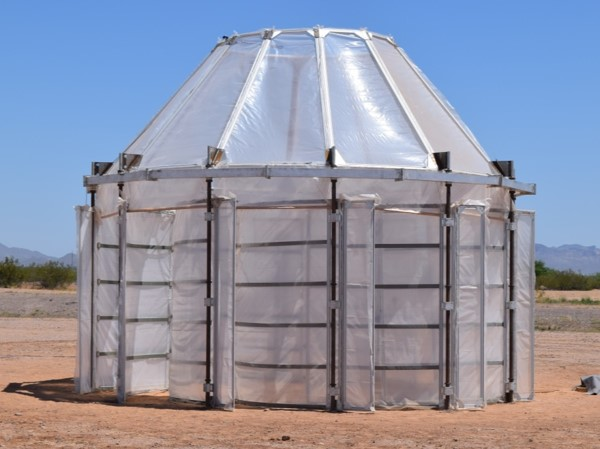
\includegraphics[width = 12 cm]{figs/sov_field}
    \caption{A photo of the field configuration, during the June 2015
    Field Test.}
    \label{fig:field_real}
   \end{center}
  \end{figure}

\todo{add energy flux calculation}

\subsection{Thermal Only}

While ambient winds in the field do impact system performance, it is
also illuminating to consider an idealized scenario with natural convection
driven only by thermal instabilities. Investigating this baseline,
thermal-only flow is intended to optimize the SoV apparatus to form a
strong thermal plume even in the absence of wind. After a system is
engineered to form a strong thermal plume, we can investigate to ensure
that the existing thermal vortex will be strengthened by the addition of
winds. 

\todo{fix these shitty figures}

  \begin{figure}[htp]
   
   \centering
   \begin{minipage}{0.47\textwidth}
    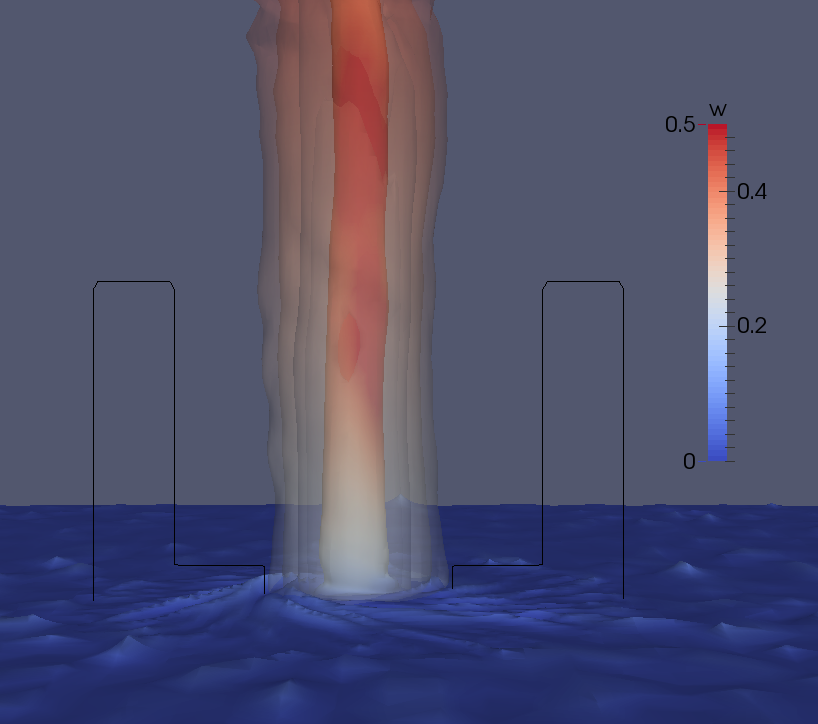
\includegraphics[width =0.9\textwidth]{figs/3d}
    \caption{This image depicts isocountours of the inner thermal core
    visible through semi-transparent contour around azimuthal velocity,
    colored by vertical velocity. }
   \end{minipage}      
   \label{fig:thermal}  

   \centering   
   \begin{minipage}{0.47\textwidth}
    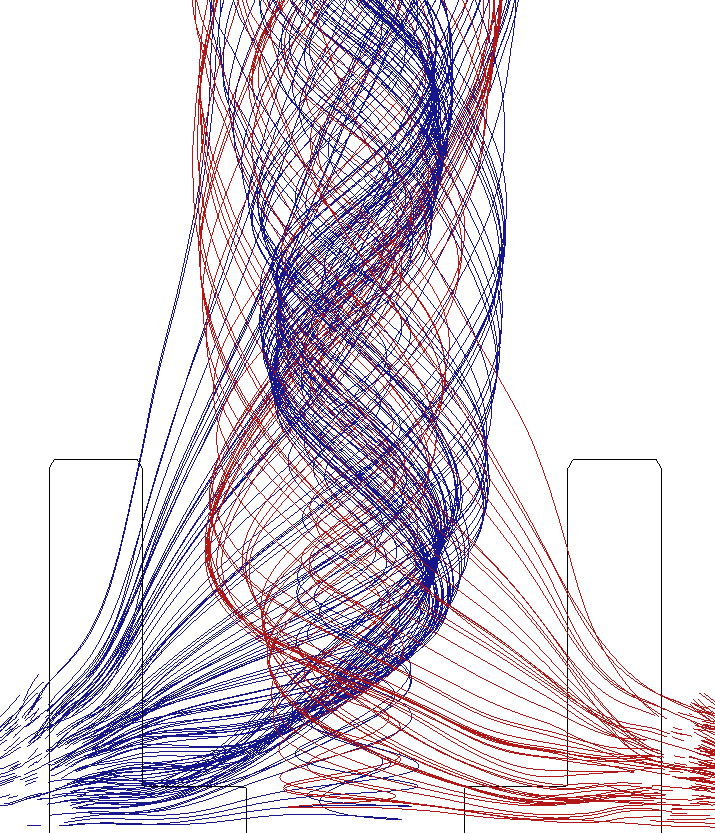
\includegraphics[width =0.9\textwidth]{figs/entrainment}%
    \caption{This is an image of particles seeded and advanced
    through a velocity field. One can observe a tight inner vortex with
    significant azimuthal velocity formed through the bottom tier of
    vanes, as well as a broader region of entrained fluid through the
    second tier.} 
   \end{minipage}   
   \label{fig:entrain}  
  \end{figure}   



In this subsection we show a representative case of an optimized thermal-only SoV
configuration. The results shown are the averages of several snapshots
from the field written over the course of several minutes. In general,
the averaging times are on the order of 20-30 wash-out times, where a
wash-out is defined as the time required for a particle at the base of
the apparatus to flow out through the top boundary. The energy flux
through the top of the vanes is roughly 53 watts. The solution
demonstrates several features characteristic of naturally occuring dust
devils. Figure \ref{fig:thermal} shows that we have formed a tight,
coherent thermal plume roughly the same size as the inner diameter of the
lower vanes. As anticipated, this hot flow is acting like a chimney,
generating a large vertical velocity which in turn entrains and draws in
outside flow. An image of the entrainment is shown in figure
\ref{fig:entrain}. 


\begin{figure}[htb]

 \begin{subfigure}{.5\textwidth}
  \centering
  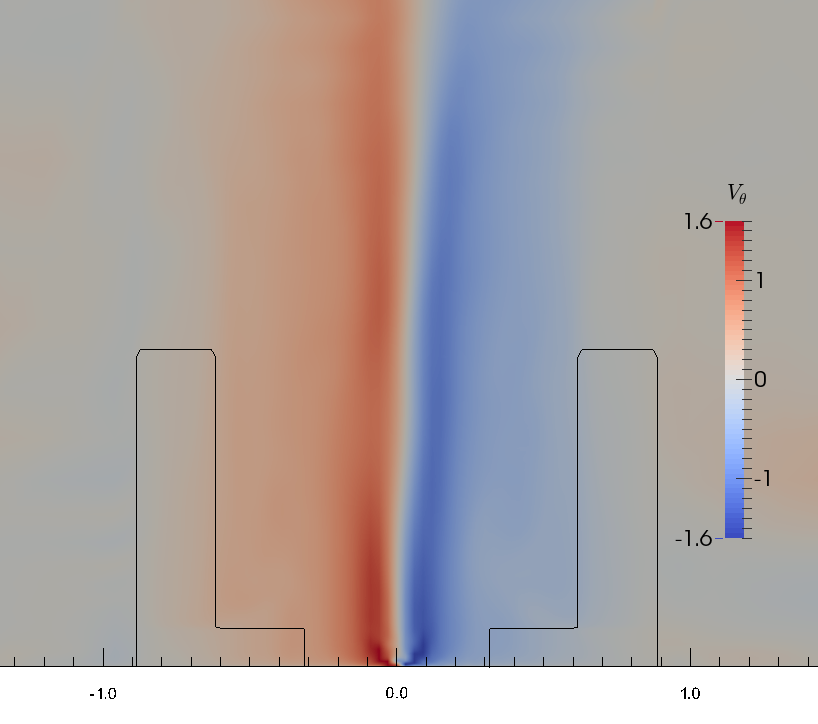
\includegraphics[width=.75\linewidth]{figs/vt}
  \caption{Azimuthal Velocity}
  \label{fig:vt-to}
 \end{subfigure}%
 \begin{subfigure}{.5\textwidth}
  \centering
  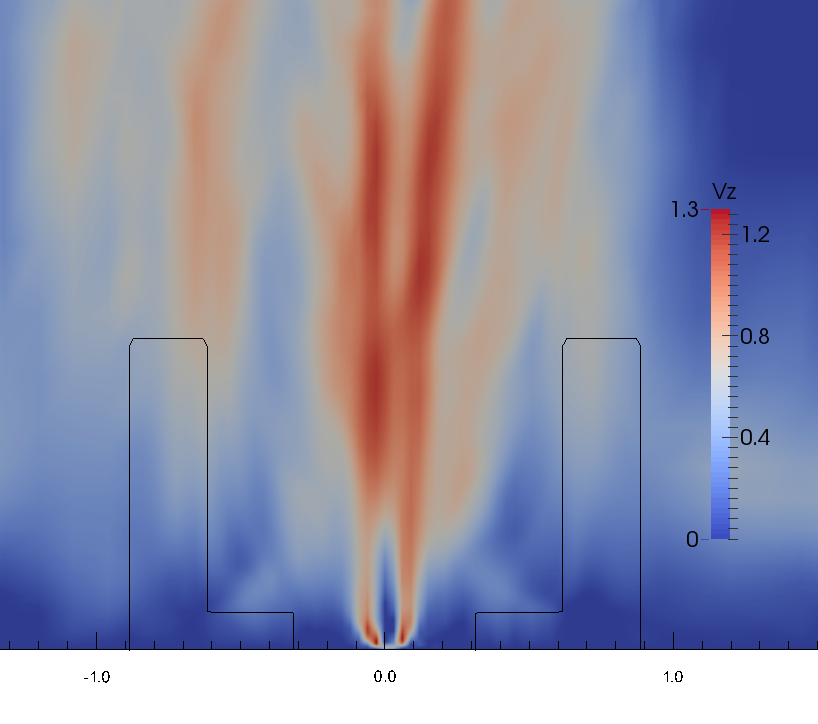
\includegraphics[width=.8\linewidth]{figs/vz}
  \caption{Vertical Velocity}
  \label{fig:vz-to}
 \end{subfigure}%


 \begin{subfigure}{.5\textwidth}
  \centering
  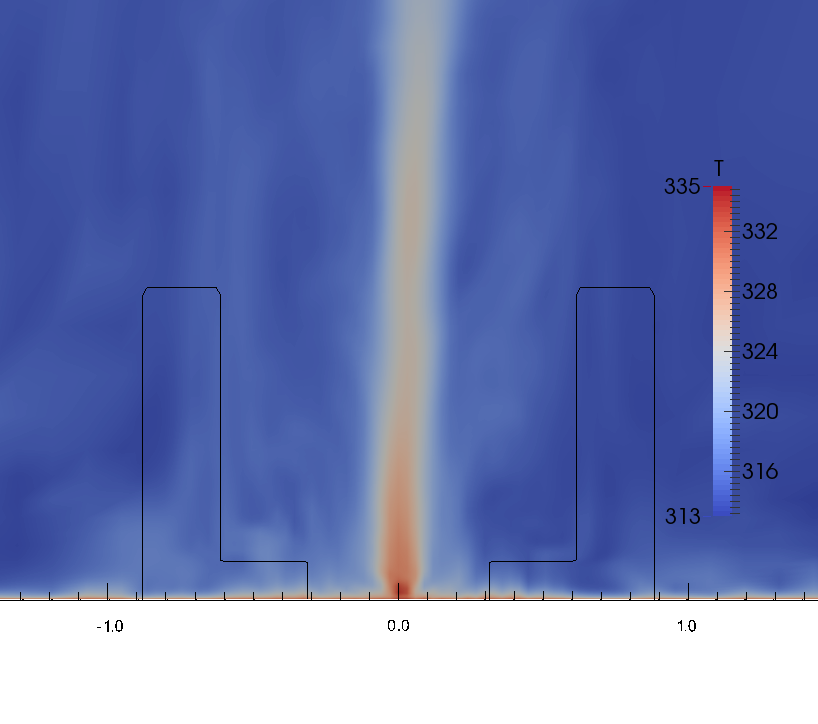
\includegraphics[width=.85\linewidth]{figs/t}
  \caption{Temperature}
  \label{fig:t-to}
 \end{subfigure}%
 \begin{subfigure}{.5\textwidth}
  \centering
  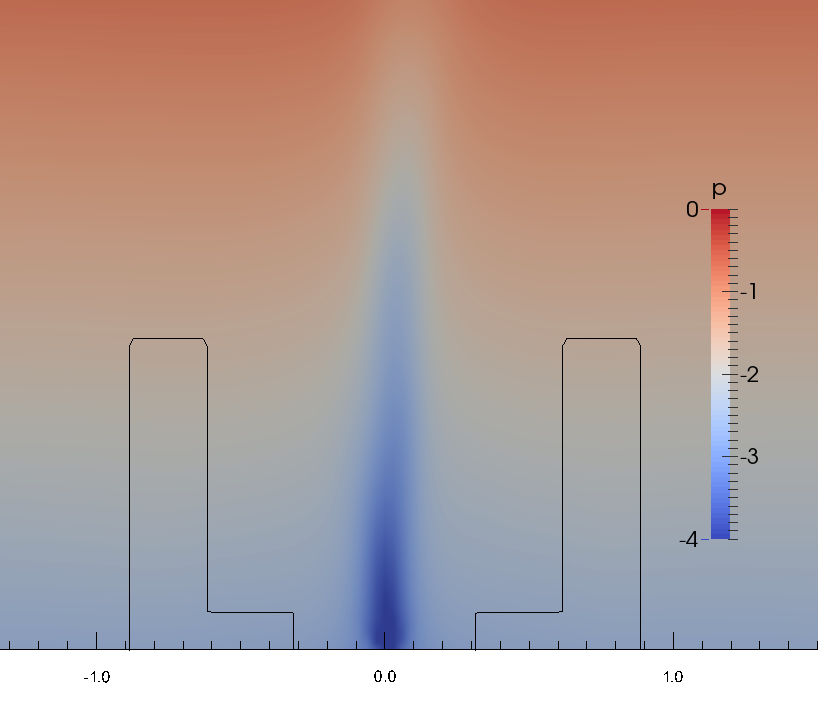
\includegraphics[width=.75\linewidth]{figs/p}
  \caption{Pressure}
  \label{fig:p-to}
 \end{subfigure}%

 \caption{Vertical slices for the thermal-only cases.}
 \label{fig:to-vert}
\end{figure}

%
%
%
Figure \ref{fig:to-vert} depicts several vertical slices through the SoV
for various state variables. One can see that there is a tight core
vortex with azimuthal and vertical velocities of several meters per
second. The tight vortex region coincides with a high temperature, low
pressure core region. On the vertical velocity plot, notice that a small
downward flow region has formed in the middle of the vortex. 

\begin{figure}[htb]

 \begin{subfigure}{.5\textwidth}
  \centering
  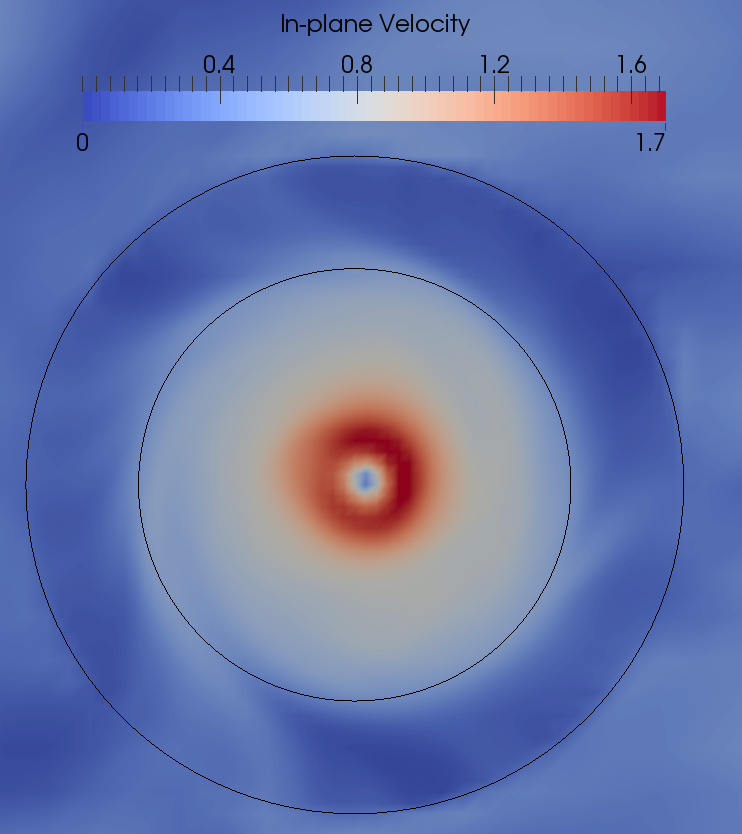
\includegraphics[width=.75\linewidth]{figs/vt_hor}
  \caption{Azimuthal Velocity}
  \label{fig:vt-to}
 \end{subfigure}%
 \begin{subfigure}{.5\textwidth}
  \centering
  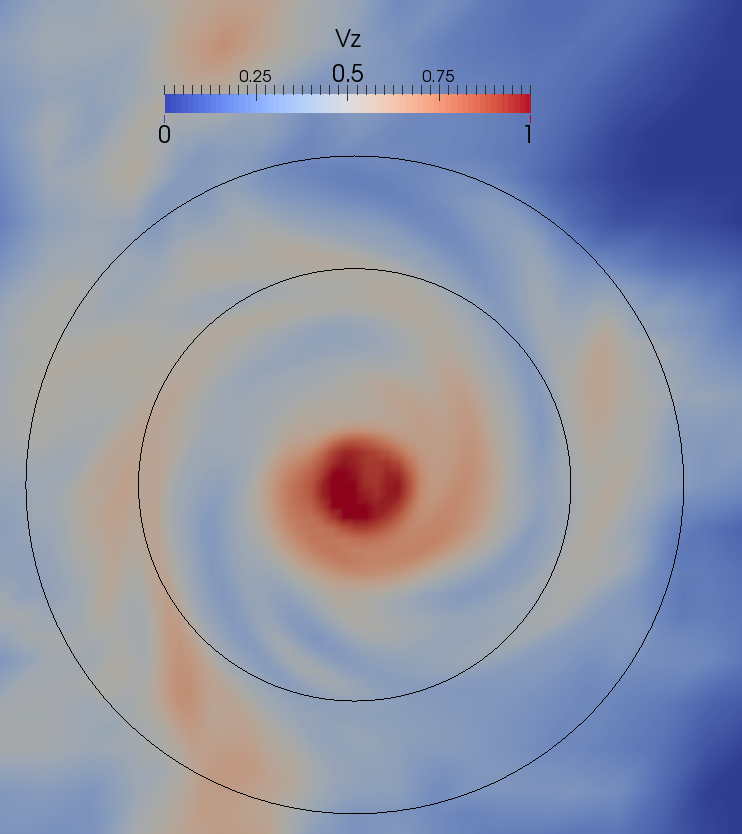
\includegraphics[width=.8\linewidth]{figs/vz_hor}
  \caption{Vertical Velocity}
  \label{fig:vz-to}
 \end{subfigure}%


 \begin{subfigure}{.5\textwidth}
  \centering
  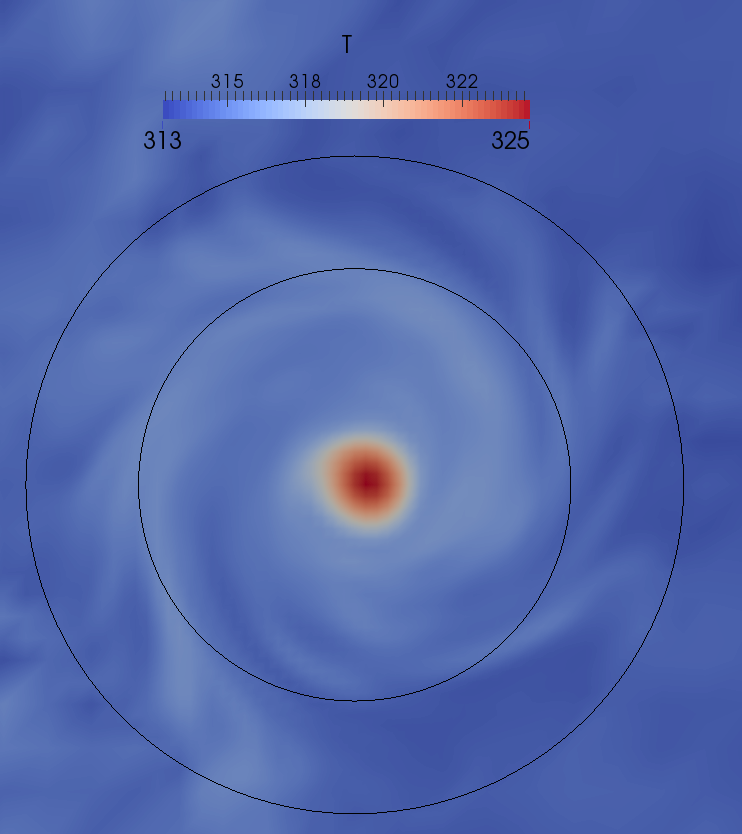
\includegraphics[width=.85\linewidth]{figs/t_hor}
  \caption{Temperature}
  \label{fig:t-to}
 \end{subfigure}%
 \begin{subfigure}{.5\textwidth}
  \centering
  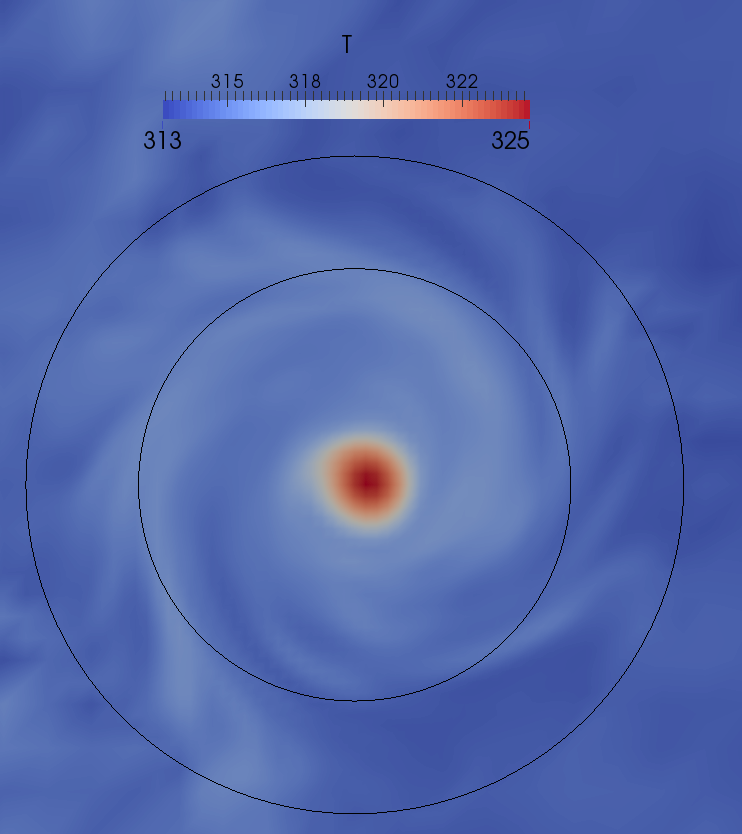
\includegraphics[width=.75\linewidth]{figs/t_hor}
  \caption{Pressure}
  \label{fig:p-to}
 \end{subfigure}%

 \caption{Horizontal slices for the thermal-only cases.}
 \label{fig:to-hor}
\end{figure}

Figure \ref{fig:to-hor}, in turn,  depicts several horizontal slices
through the SoV for the same state variables. It can be seen that the
large velocities are highly limited to a region just inside the
vanes. Likewise, the entrainment of fluid is limited to a region
immediately surrounding the vanes. 
%
% conclusion of thermal only
%
Finally, the thermal plume is relatively
narrow compared to the diameter of the device. It is desirable to
broaden the thermal plume, as this in turn creates a larger vertical
momentum flux due to the effects of buoyancy. This will presumably
entrain more surrounding fluid, driving it through the vanes and
imparting kinetic energy to the flow. The kinetic energy grows as the
square of the radius, so any broadening of the vortex core can greatly
enhance the kinetic energy flux. The diameter of the thermal core is
therefore a critical driver to the energy of the thermal-only
conditions, and operates as the ``prime-mover'' of the entire
process. Broadening this plume will necessarily enhance the energy
flux that can be extracted. However, the general physical
mechanisms that determine the thermal plume's thickness are not
presently understood. 


 \todo{fix these images}
These slices lend credibilty to the notion that our turning vane
configuration is generating something with parallels to a real dust
devil.   


Rotating air induces low pressure core, as observed in:
Dust Devils

\subsection{Wind}

Potential Temperature is defined as,\todo{where are you using this fellow}
\begin{equation}
  \theta(x,y,z) = T(x,y,z) -T_{in}(z) 
\end{equation}

Discussion thermal + wind

\subsection{Optimization}

In this section we show results from a representative optimization
effort for a thermal-only case, in order to detail the mode of operation
these efforts have presently followed. 

typical mode of scientific and engineering inquiry, which is to say
hypothesis of system operation followed by testing and then evaluation
and possibly, validatio of the testing. 

image of vanes before after

image of flow before after

table of energy flux increase